\documentclass{article}

\usepackage[margin=0.5in]{geometry}

\usepackage{graphicx}
\usepackage{caption}
\usepackage{subcaption}

\usepackage{cleveref}

\title{CE EN 507: Coding Assignment 2}
\author{ Jared J.~Thomas}

\begin{document}
\maketitle

\section{Part 1}
Please see attached file, fem.py, for my nD FEM code.

\section{Part 2}
\subsection{}
The parameters chosen for this problem are shown in \cref{tab:parameters}. For Part 2, $A_S$ was used for $A$.

\begin{table}
	\centering
	\begin{tabular}{| r | r |}
		\hline
		$L$ & 1.0 \\
		$N$ & 10.0 \\
		$E$ & 200E9 \\
		$A_{S}$ & 2.5E-5\\
		$A_{L}$ & 100 \\
		$I_1$ & 5.21e-11\\
		$I_2$ & 5.21e-11\\
		$J$ & 1.04e-10\\
		$\nu$ & 0.3 \\
		$G$ & 76.9E9 \\
		\hline
	\end{tabular}
	\caption{Parameters and other relevant values}
	\label{tab:parameters}
\end{table}

\subsection{}
The maximum displacement at the right end of the beam using an analytic approach was 9.99999333611E-7.

\subsection{}
Please refer to \cref{fig:part2} for a plot of computed displacements for Part 2.

\begin{figure}[ht]
	\centering
	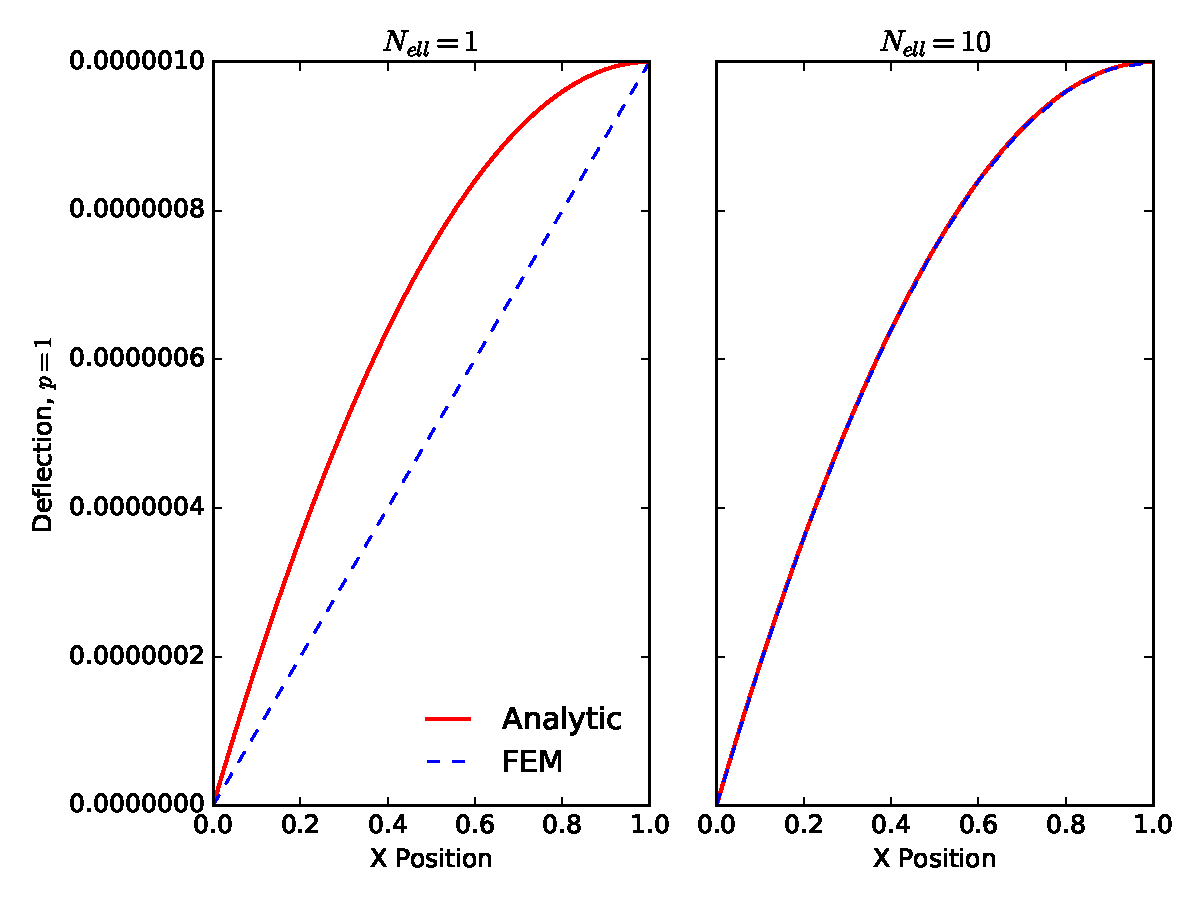
\includegraphics[width=0.75\textwidth]{beam1_deflection_prob2_dof2}
	\caption{Deflection plot for Part 2}
	\label{fig:part2}
\end{figure}

\subsection{}
The maximum displacement at the right end of the beam using my FEM code was 1E-6, which is essentially equal to the analytic solution (9.99999333611E-7).

\section{Part 3}

\subsection{}
Refer to \cref{tab:parameters} for parameter and other values used in this section.

\subsection{}
Please see \cref{fig:31,fig:32} for plots of $u^h(x)$ and $\theta^h(x)$ versus the exact solution $u(x)$ and $\theta(x)$.

\begin{figure}[ht]
	\centering
	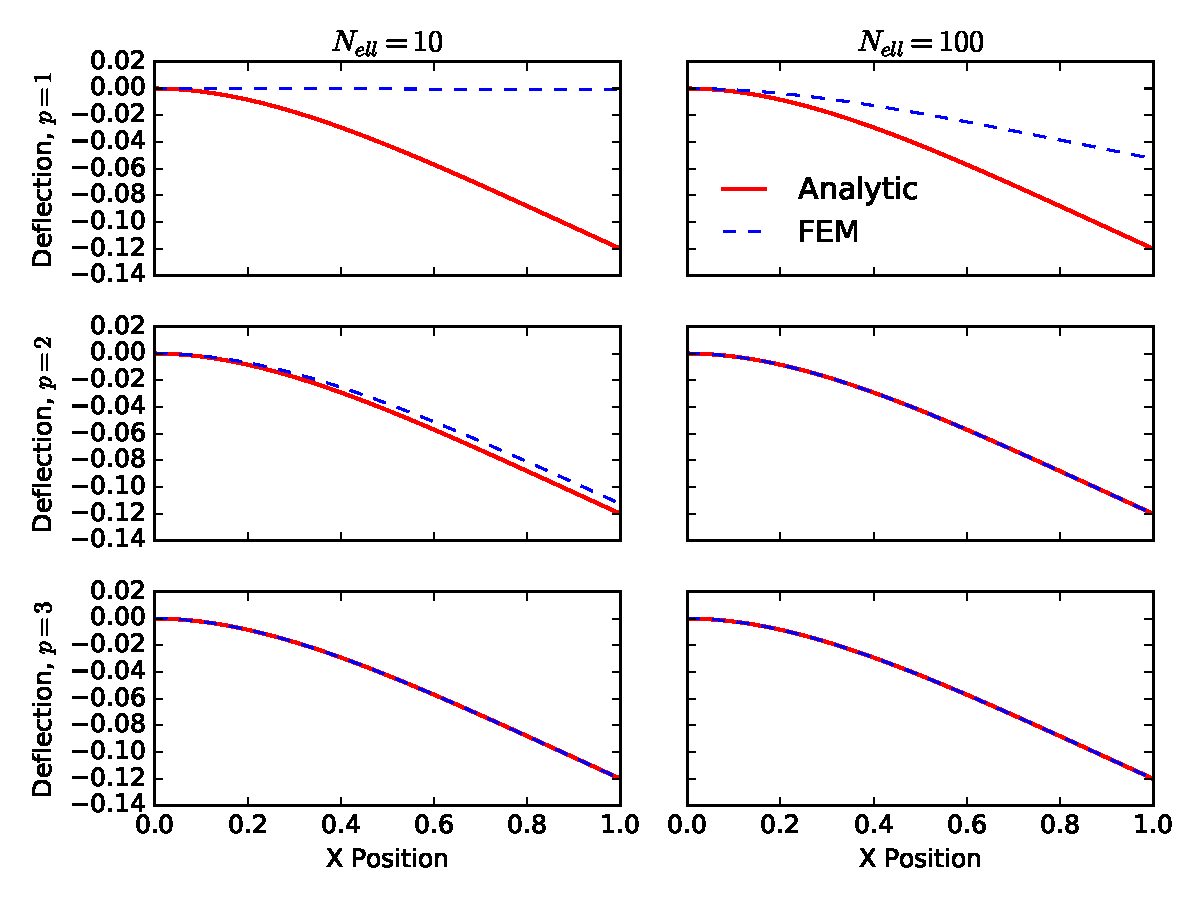
\includegraphics[width=0.75\textwidth]{beam1_deflection_prob3_dof0}
	\caption{$u^h(x)$ versus $u(x)$ for Part 3}
	\label{fig:31}
\end{figure}

\begin{figure}[ht]
	\centering
	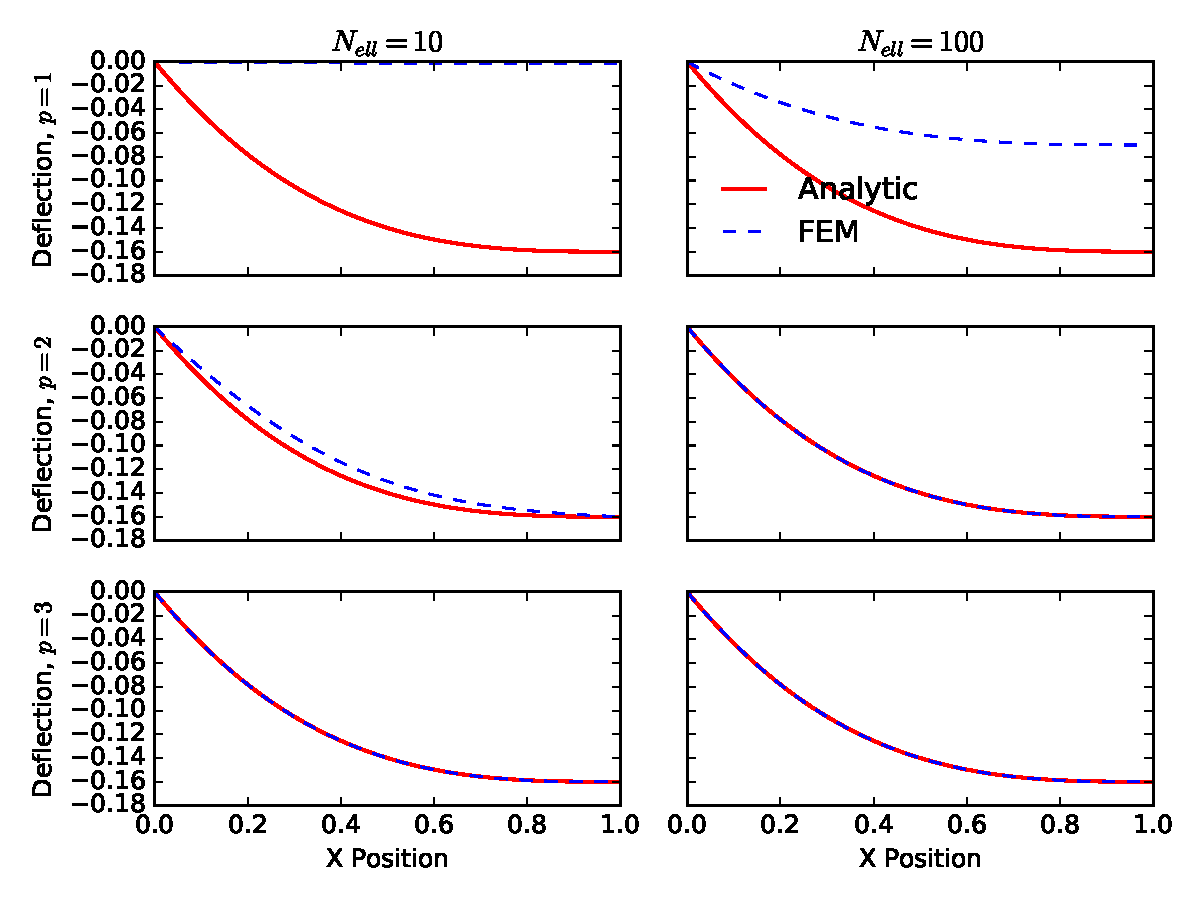
\includegraphics[width=0.75\textwidth]{beam1_deflection_prob3_dof4}
	\caption{$\theta^h(x)$ and $\theta(x)$ for Part 3. For p=1 and N=10, the FEM deflection is essentially zero}
	\label{fig:32}
\end{figure}

\subsection{}
For this part, $A_S$ was used for the thin beam, and $A_L$ was used for the thick beam. (See \cref{tab:parameters}. Results for the thin beam were as follows: $u^h_{max} = 0.118403120283$, $u_{max} = 0.1232000064$, $\theta^h_{max} =  0.15999984117 $, and $\theta_{max} = 0.16000128$. Results for the thick beam were as follows: $u^h_{max} = $7.87322000026E-13, $u_{max} = $7.7000004E-15, $\theta^h_{max} = $9.99999E-15, and $\theta_{max} = $1.000008E-14. It can be easily seen that the results for the thick beam for FEM and the analytic solution differed by an order of magnitude. This discrepency is due to the thin beam assumptions made to solve the problem as a beam problem.

\section{Part 4}

\subsection{}
Refer to \cref{tab:parameters} for parameter and other values used in this section.

\subsection{}
Please see \cref{fig:41,fig:42} for plots of $u^h(x)$ and $\theta^h(x)$ versus the exact solution $u(x)$ and $\theta(x)$.

\begin{figure}[ht]
	\centering
	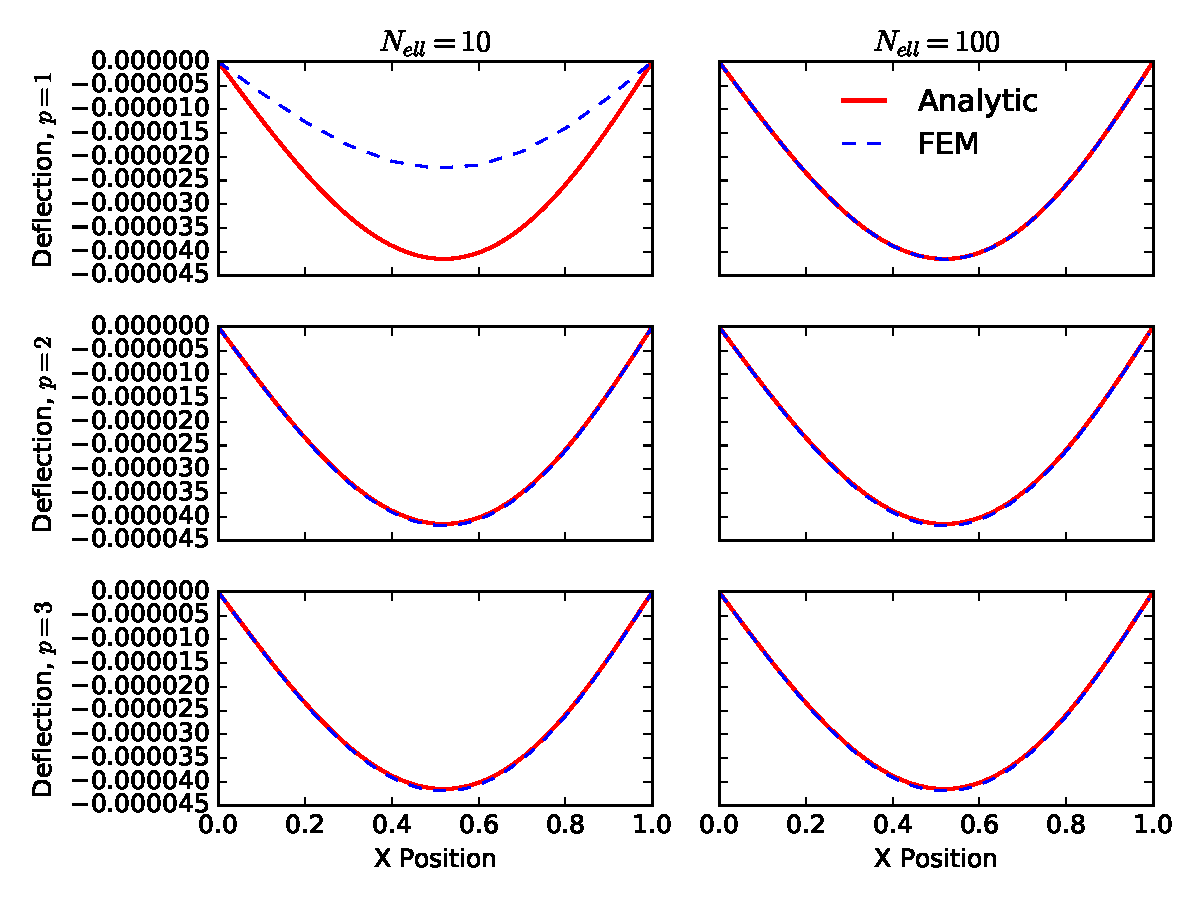
\includegraphics[width=0.75\textwidth]{beam1_deflection_prob4_dof0}
	\caption{$u^h(x)$ versus $u(x)$ for Part 4}
	\label{fig:41}
\end{figure}

\begin{figure}[ht]
	\centering
	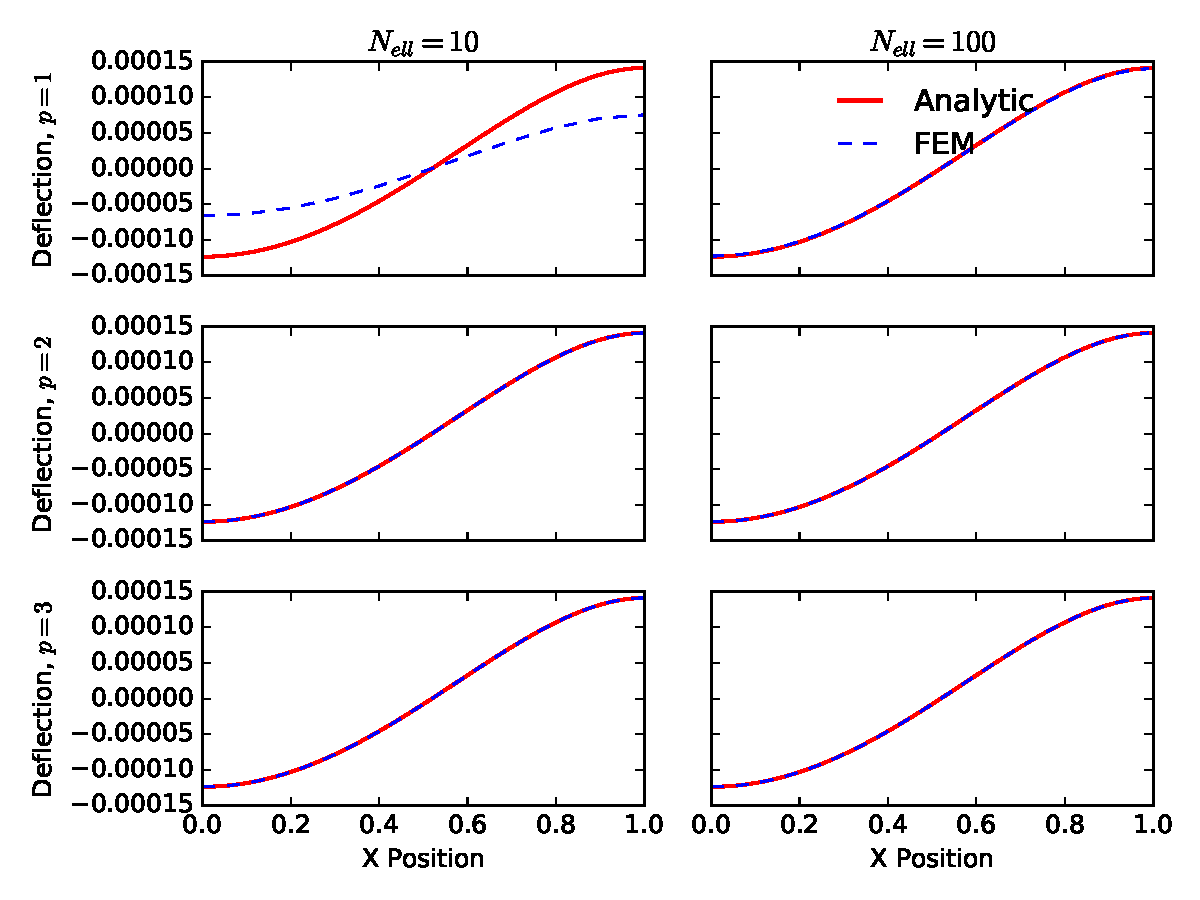
\includegraphics[width=0.75\textwidth]{beam1_deflection_prob4_dof4}
	\caption{$\theta^h(x)$ and $\theta(x)$ for Part 4}
	\label{fig:42}
\end{figure}


\end{document}